
\documentclass[letterpaper]{article}
\usepackage{aaai}
\usepackage{times}
\usepackage{helvet}
\usepackage{algorithm}
\usepackage{algpseudocode}
\usepackage{courier}
\usepackage{graphicx}
\graphicspath{{./figure/}}
\frenchspacing
\setlength{\pdfpagewidth}{8.5in}
\setlength{\pdfpageheight}{11in}
\begin{document}    

\section{Objects Representation with the extended GSR-n (EGSR)} 
\section{Objects Representation with the extended GSR-n (EGSR)} 

We use a minimum bounding rectangle (MBR) to approximate the region occupied by a circle and use exact shapes for the general solid rectangles (GSR), i.e. rectangles that can have any angle and impenetrable. 

Many rectangle-based spatial calculi \cite{balbiani1998model,cohn2012thinking,sokeh2013efficient} are developed in the context of Qualitative Spatial Reasoning \cite{cohn2001qualitative} for dealing with different spatial aspects of such as topology, size etc. One of them is GSR-n, proposed by \cite{Ge2013}. GSR-n is a comprehensive spatial representation of GSRs. It defines eight contact sectors that correspond to the eight edges and corners of the rectangles. Given two GSRs $o_1$ and $o_2$ that contact each other via $sector_1, sector_2 \in \{S_1, ..., S_8, R_1, ..., R_8\}$, the contact relation between $o_1$ and $o_2$ can be expressed as the constraint $o_1 \, (sector_1, sector_2) \, o_2$ (Figure \ref{GSR}). With the contact relations, GSR-n allows us to distinguish if and how two objects contact each other. Since the objects can only interact via contacts, we can further infer the possible motions of an object from the GSR relations the object holds with others. GSR-n also defines a set $n$ of unary relations by the $Qualitative\,Corner\,Instantiations$, which qualitatively describes the size and leaning direction of a GSR. Since we represent the rectangles using real shapes, we do not need the unary relations. 
\begin{figure}[h!]
\centering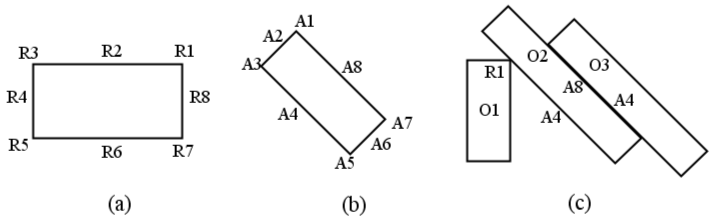
\includegraphics[scale=0.25]{GSR.png}\caption{Contact sectors of (a) a normal rectangle (without rotation) and (b) an angular rectangle. (c) An example scenario where $o_1 (R_7, S_4) o_2$, $o_2 (S_8, S_4) o_3$}
\label{GSR}
\end{figure}


Given two GSRs, we obtain the contact relation by enumerating all the plausible combinations of the two GSRs' contact sectors and for each combination calculating the distance between the two sectors. The combination with the shortest distance constitutes the contact relation. Note, the shortest distance can be non-zero. A non-zero distance means the two GSRs are separate, otherwise touch. So unlike the original definition that the contact relation can only be assigned when two GSRs touch, here we can assign a contact relation for any pair of GSRs. To distinguish whether two GSRs touch or not, we turn to qualitative distance which is covered in the next section.
\begin{figure}[h!]
\centering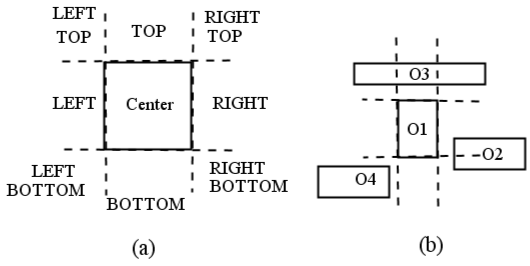
\includegraphics[scale=0.35]{CardinalTiles.png}\caption{(a) The nine cardinal tiles (b) An example scenario where $o_3 (TOP) o_1$, $o_2 (RIGHT) o_1$, and $o_4 (BOTTOM\,LEFT) o_1$}
\label{CardinalTile}
\end{figure}
The problem with GSR-n is that it uses $(\emptyset, \emptyset)$ to represent the spatial relation between all the non-touched GSRs. Thus, it introduces ambiguities when the rectangles are disconnected. To overcome the ambiguities, we extend the original GSR-n by integrating it with the cardinal tiles \cite{goyal1997direction}. Specifically, we partition the embedding space around an reference object into nine mutually exclusive tiles(see Figure \ref{CardinalTile}.a). The centre tile corresponds to the minimum bounding rectangle of the object and the other eight tiles correspond to the eight cardinal directions. We call the $LEFT$, $RIGHT$, $BOTTOM$, $TOP$ core tiles.  

\begin{figure}[h!]
\centering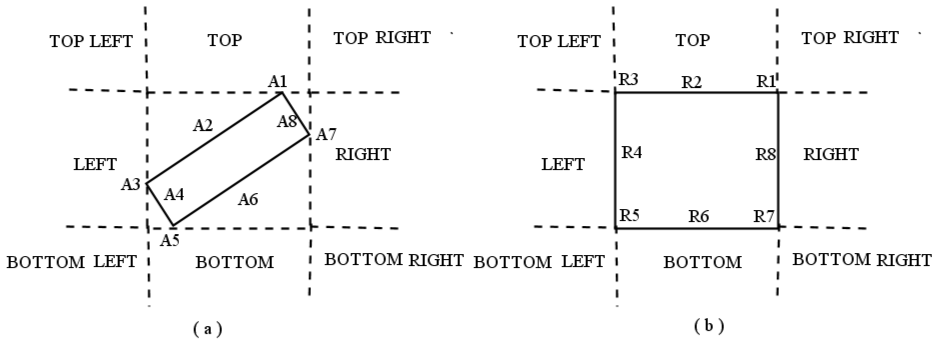
\includegraphics[scale=0.25]{EGSR-relations.png}\caption{Contact sectors and Cardinal directions of (a) an angular rectangle and (b) a normal rectangle}
\label{EGSR}
\end{figure}
The new representation is called EGSR (see Figure \ref{EGSR}). Given a set ${\cal B}_{GSR}$ of GSR contact relations and a set ${\cal B}_{card}$ of cardinal tiles,  we add $\bot$ to both sets to indicate a unassigned relation, an EGSR relation is then written as $(r_1, r_2), r_1 \in {\cal B}_{GSR}\cup \{\bot\}, r_2 \in {\cal B}_{card}\cup \{\bot\}$. We abbreviate $(r_1,r_2)$ by the cardinal tile $r_2$ or by the contact relation $r_1$ if it is clear which one is meant. 

We compute the EGSR relation between two spatial objects by first checking whether their MBRs intersect or boundary touch. If so, we assign a GSR-n relation accordingly. Otherwise, one of the eight cardinal tiles will be used. If one object's MBR occupies multiple tiles of the referred object, we will assign the core tile occupied by the MBR (see Figure \ref{CardinalTile}.b). Note, when one object's MBR occupies more than one core tiles of the referred object, it must intersect or boundary touch the referred object's MBR, in this case, GSR-n relation will be assigned instead. All EGSR relations are obviously converse, e.g. the converse of $TOP\,LEFT$ is $BOTTOM\,RIGHT$, the converse of $(R_4, S_1)$ is $(S_1,R_4$).

\cite{wallgrun2010qualitative} introduced the notion of qualitative interpretation that extracts qualitative descriptions from the input data. A scenario containing multiple spatial objects can be qualitatively interpreted by EGSR via a qualitative constraint network (QCN). QCN is a labelled graph where each node corresponds to an object and directed edges represents relational constraint that has to hold between the two objects. 
Figure \ref{QCN} shows an example of a QCN based on EGSR relations.

 \begin{figure}[h!]
\centering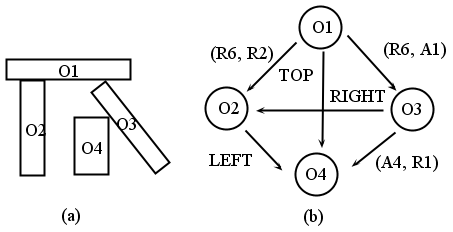
\includegraphics[scale=0.45]{QCN.png}\caption{(a) A spatial scenario where the four rectangles form a stable structure under downward gravity (b) The corresponding qualitative constraint network}
\label{QCN}
\end{figure}
\end{document}